\subsection{Li-Ion-Batterie}\label{sec:energiespeicher}

Die gesamte Energiespeicherung erfolgt durch einen Lithium-Ionen-Akkumulator des Typs Emmerich LI14500. Dieser weist eine Kapazität von $800mAh$ bei einer Nominalspannung von $3.7V$ auf. Ausserdem weist der Akkumulator integrierte Schutzeinrichtungen auf, welche später im Abschnitt \nameref{sec:schutzeinrichtung} (Kapitel \ref{sec:energiespeicher}) weiter erläutert werden. Um eine Abschätzung über die Betriebszeit des Dōjōs zu erhalten, sind Faktoren wie maximaler Verbrauch, Nominalspannung und Kapazität notwendig. Die maximale Leistung des Dōjōs lässt sich durch die Leistung des Knochenschallgebers und die des Microcontrollers beschreiben. Alle anderen Komponenten können durch ihren geringen Betriebsstrom durch einen Sichheitsfaktor von $0.1W$ dazu gerechnet werden. Die Leistung des Verstärkers welcher den Knochenschallgeber speist, weist eine maximale RMS Leistung von $471.9mW$ auf. Die Rechnung erfolgt mit $80\%$ des RMS Wertes, da der Knochenschallgeber nicht rund um die Uhr angesprochen wird. Die Microcontrollerleistung ergab durch tests im Labor eine Leistung von 27.36mW. Nachfolgende Berechnung \ref{eq:MaxLeistung} gibt einen Einblick in die Gesamtleistung.

\begin{equation}
\centering
P_{max}=\left(0.8\cdot P_{Kn}\right)+P_{MC}+P_{zus}=(0.8\cdot 0.472W)+(0.02736W)+0.1W=0.506W
\label{eq:MaxLeistung}
\end{equation}

Die Gesamtleistung beträgt somit rund 0.506W. Um die daraus folgende minimale Zeit t zu berechnen, gilt nachfolgende Berechnung \ref{eq:Betriebszeit}.

\begin{equation}
\centering
t_{max}=\frac{W\cdot U}{P_{tot}}=\frac{800mAh \cdot 3.7V}{506mW}=5.85h\approx 5h \thickspace 51min
\label{eq:Betriebszeit}
\end{equation}

Bei ständigem Gebrauch kann somit eine minimale Betriebszeit von knapp 6 Stunden erreicht werden. Hierbei gilt es zu erwähnen, dass durch einen geschickten Ladeprozess (gemäss Kapitel \ref{sec:anwendung}) ein lückenloser Betrieb garantiert werden kann.


\subsubsection*{Schutzeinrichtungen}\label{sec:schutzeinrichtung}
Um den verwendeten Akkumulator zu schützen, sind diverse Schutzeinrichtung notwendig. Zum einen muss der Ladevorgang überwacht werden, so dass der maximale Ladestrom wie auch die Ladespannung nicht überschritten werden. Für die Laderegelung wurde ein Lade-IC von Microchip des Typs MCP73831 verwendet. Dieser übernimmt die gesamte Spannungs- und Stromregelung beim Ladeprozess und kann zu dem während dem Ladevorgang eine LED zur Ladesignalisation ansteuern. Der Ladeprozess für den oben erwähnten Li-Ion Akku ist in untenstehender Abbildung  \ref{fig:Ladekurve Li-Ion Akku} ersichtlich. Hierbei wurde der Akku im Schnelllademodus mit einem maximalen Strom von 400mA geladen. Dieser Strom ergibt sich aus dem Datenblatt der Batterie, wobei sowohl der Entladestrom, als auch der Ladestrom 0.5C beträgt. Das C entspricht der Kapazität der Batterie, wodurch sich der Strom Imax gemäss der nachfolgenden Formel \ref{eq:Ladestrom} berechnen lässt.

\begin{equation}
\centering
I_{charge}={\frac{0.5}{h} \cdot C}={\frac{0.5}{h} \cdot 800mAh}=0.4A\thickspace \widehat {=} \thickspace 400mA
\label{eq:Ladestrom}
\end{equation}

Betrachtet man die Abbildung \ref{fig:Ladekurve Li-Ion Akku}, so wird ersichtlich, dass die Spannung rund $2.5h$ geregelt wird bis 4.2V Grenze erreicht wird. Sobald der Spannungswert $4.2V$ erreicht hat, beginnt der Lade-IC mit der Stromregelung. Für diesen Prozess wurden beim Versuch noch einmal rund 30 Minuten benötigt, wodurch die letzten rund $20\%$ der Batteriekapazität geladen werden konnten.

\begin{figure}[H]
	\begin{center}
		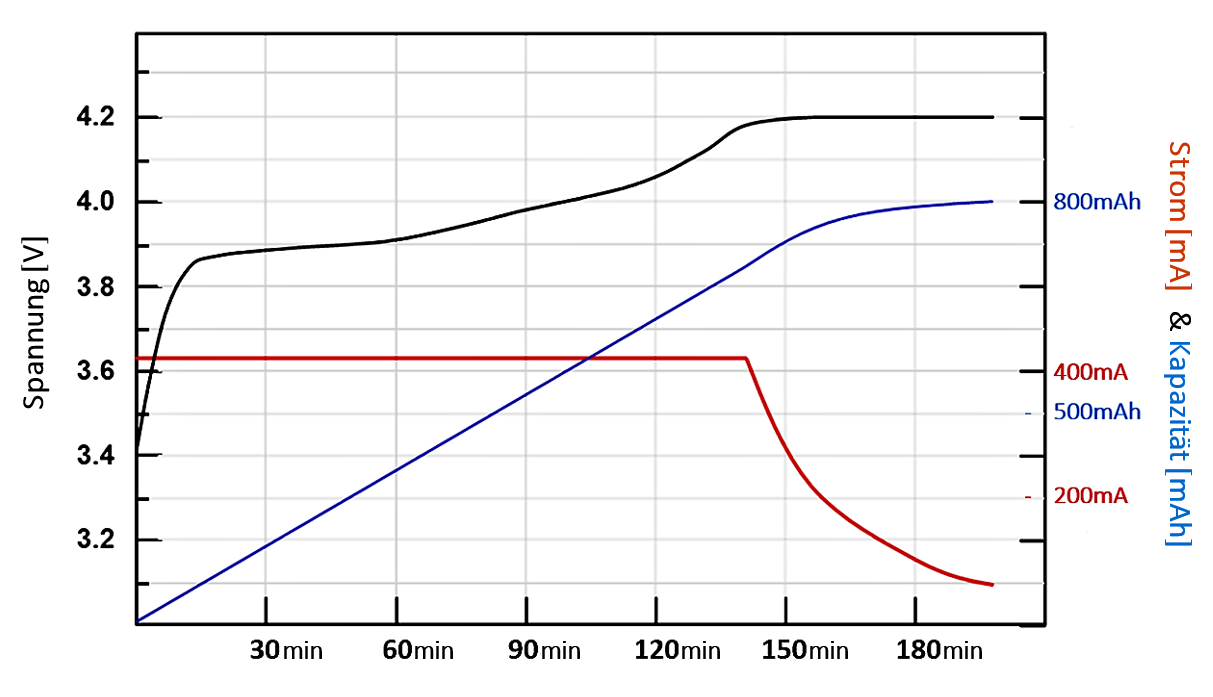
\includegraphics[width=120mm]{data/LadekurveLiIon.png}
		\caption[Blockschaltbild Energiespeicherung]{Blockschaltbild Energiespeicherung} %picture caption
		\label{fig:Ladekurve Li-Ion Akku}
	\end{center}
\end{figure}


Für einen weiteren Schutz, hat die Emmerich LI14500 eine integrierte Schutzbeschaltung namens PCM (Protection Circuit Module). Dieser Schutz garantiert einerseits einen Überladeschutz von $4.25V\pm 0.025V$, aber auch einen Tiefentladungsschutz von $2.5V\pm 0.063V$. Weiter ist der Akku gegen Überströme ab einer Höhe von 4.8A geschützt und weist zudem einen Schutzschaltungswiderstand von $\leq 75mW$ auf. Das Testing des integrierten Schutzschaltung findet in der Hardware Validierung \ref{sec:testkonzeptHardware} statt.

